\documentclass[man,a4paper,noextraspace,apacite]{apa6}\usepackage[]{graphicx}\usepackage[]{color}
%% maxwidth is the original width if it is less than linewidth
%% otherwise use linewidth (to make sure the graphics do not exceed the margin)
\makeatletter
\def\maxwidth{ %
  \ifdim\Gin@nat@width>\linewidth
    \linewidth
  \else
    \Gin@nat@width
  \fi
}
\makeatother

\definecolor{fgcolor}{rgb}{0.345, 0.345, 0.345}
\newcommand{\hlnum}[1]{\textcolor[rgb]{0.686,0.059,0.569}{#1}}%
\newcommand{\hlstr}[1]{\textcolor[rgb]{0.192,0.494,0.8}{#1}}%
\newcommand{\hlcom}[1]{\textcolor[rgb]{0.678,0.584,0.686}{\textit{#1}}}%
\newcommand{\hlopt}[1]{\textcolor[rgb]{0,0,0}{#1}}%
\newcommand{\hlstd}[1]{\textcolor[rgb]{0.345,0.345,0.345}{#1}}%
\newcommand{\hlkwa}[1]{\textcolor[rgb]{0.161,0.373,0.58}{\textbf{#1}}}%
\newcommand{\hlkwb}[1]{\textcolor[rgb]{0.69,0.353,0.396}{#1}}%
\newcommand{\hlkwc}[1]{\textcolor[rgb]{0.333,0.667,0.333}{#1}}%
\newcommand{\hlkwd}[1]{\textcolor[rgb]{0.737,0.353,0.396}{\textbf{#1}}}%

\usepackage{framed}
\makeatletter
\newenvironment{kframe}{%
 \def\at@end@of@kframe{}%
 \ifinner\ifhmode%
  \def\at@end@of@kframe{\end{minipage}}%
  \begin{minipage}{\columnwidth}%
 \fi\fi%
 \def\FrameCommand##1{\hskip\@totalleftmargin \hskip-\fboxsep
 \colorbox{shadecolor}{##1}\hskip-\fboxsep
     % There is no \\@totalrightmargin, so:
     \hskip-\linewidth \hskip-\@totalleftmargin \hskip\columnwidth}%
 \MakeFramed {\advance\hsize-\width
   \@totalleftmargin\z@ \linewidth\hsize
   \@setminipage}}%
 {\par\unskip\endMakeFramed%
 \at@end@of@kframe}
\makeatother

\definecolor{shadecolor}{rgb}{.97, .97, .97}
\definecolor{messagecolor}{rgb}{0, 0, 0}
\definecolor{warningcolor}{rgb}{1, 0, 1}
\definecolor{errorcolor}{rgb}{1, 0, 0}
\newenvironment{knitrout}{}{} % an empty environment to be redefined in TeX

\usepackage{alltt}
\usepackage{apacite}
\title{What Does Perspective Taking Do for Vicarious Emotions?}
\shorttitle{Perspective Taking}
\author{Joshua D. Wondra and Phoebe C. Ellsworth}
\affiliation{University of Michigan}

\abstract{Abstract TBD}
\keywords{empathy, vicarious emotions, perspective taking}

\authornote{Joshua D. Wondra, Department of Psychology, University of Michigan.

Phoebe C. Ellsworth, Department of Psychology, University of Michigan.

Correspondence concerning this article should be addressed to Josh Wondra, Department of Psychology, University of Michigan, 530 Church St., Ann Arbor, MI 48109-1043.

Contact: jdwondra@umich.edu}
\IfFileExists{upquote.sty}{\usepackage{upquote}}{}
\begin{document}

\maketitle

\section{Method}



\subsection{Overview}

    Subjects read a bogus letter from another person who described an emotional experience that made her feel sad or angry. Subjects were told that while reading the letter they should take the other person's perspective, remain objective, or they received no specific instructions as a control condition. Thus, the study had a 2 (Target's Emotion: sad, angry) x 3 (Instructions: perspective taking, objective, control) between-subjects factorial design. Initially we only ran subjects in the perspective taking and objective conditions, but we decided to add the control condition to clarify what differences could be attributed to perspective taking and what differences could be attributed to regulating one's emotions by remaining objective. Then subjects reported their own emotions, their perceptions of the letter writer's emotions, their appraisals of the letter writer's situation, and their perceptions of the letter writer's appraisals of the situation.
    
\subsection{Subjects}

    Subjects were 329 (200 women, 126 men, 3 did not report gender) undergraduate students and community members who participated for course credit or \$5. Data from an additional 21 subjects were excluded because they were non-native English speakers, they were inattentive, or they suspected that the letter they read was not real. Subjects ages ranged from 18 to 18 (Median = 19). There were 220 who identified as European American or White, 76 who identified as Asian or Asian American, 17 who identified as African American or Black, 14 who identified as Middle Eastern, 11 who identified as Latino or Hispanic, 3 who identified as Native American or Alaska Native, 3 who identified as Native Hawaiian or Other Pacific Islander, and 4 who identified as having another racial or ethnic heritage. To indicate socieconomic status, subjects reported their parents' highest forms of education completed (see Table 1).
    
\begin{table}
  Table 1
  
  \textit{Subjects' Parents' Education as an Indicator of Socioeconomic Status}

  \begin{tabular}{l c c}
     \hline
     & Mother's Education & Father's Education \\
     \hline
     Less than high school & 
        4 (1\%) & 
        7 (2\%) \\
     High school diploma/GED & 
        22 (7\%) & 
        24 (7\%) \\
     Some college & 
        30 (9\%) & 
        27 (8\%) \\
     Associate's degree & 
        23 (7\%) & 
        8 (2\%) \\
     Bachelor's degree & 
        136 (42\%) & 
        98 (30\%) \\
     Postgraduate degree (e.g., Master's, PhD, JD, MD) & 
        111 (34\%) & 
        162 (50\%) \\
     \hline
  \end{tabular}

\end{table}

\subsection{Procedure}
Each subject participated in the study individually and was seated at a computer. They were told that the study was about how people communicate about personal experiences and react to others' personal experiences. They were told that they would begin the study by writing about a personal experience to a future participant and then they would read about the personal experience of someone else who participated in the study earlier in the semester.

Next, subjects received a pen, a piece of paper, and an envelope. They were told to write a letter to a future participant about a personal experience, and that they could write a paragraph about something interesting that happened to them recently. Then they could put their letter in the envelope when they finished writing. 

Next, the participant told the subject that they would read a randomly selected letter from somoene who participated earlier in the semester. Then the subject would complete a questionnaire on the computer about their reactions to the letter. Subjects in the perspective taking and objective conditions were told the researchers found that the way they read the letter was important. Those in the perspective taking condition were told to "try to imagine how the other person feels about what is described. Try to imagine how it has affected her life and how she feels as a result," whereas those in the objective condition were told to "try not to get caught up in how the other person feels; just remain objective and detached" \cite{Batson2002, Batson2007}.

Then the subject read a letter from another participant, Melissa, who was upset about missing her best friend's bachelorette party in New York City due to car problems. Each subject was randomly assigned to read a letter where the car problems were due to bad luck and Melissa felt sad, or where the car problems were her friend's fault and Melissa felt angry. The sad (\textit{angry}) letter read:

\begin{quote}
Dear future participant,

    So I'm supposed to write about something interesting that happened to me recently. Well, a couple of weeks ago I tried to go on a road trip with a friend, but couldn't go because of bad circumstances \textit{(because of my friend who was supposed to drive)}. My best friend of 10 years is getting married in two months and she asked me to be her maid of honor, so of course I got to plan her bachelorette party. We always wanted to visit New York City together so that was the perfect place for us to do it. One of my friends here wanted to visit his friends in NYC that weekend so he offered to drive us both. He was having some car troubles so I asked if he would be able to get it fixed before the trip or if I should try to find another way to get there. He told me that he took the car in for repairs and we were all set, so we left a few days later. Then suddenly, when we were a quarter of the way there, his car started making noises and it just died. So it turns out that he got the car fixed but the replacement part was defective \textit{(he didn't get the car fixed and he had lied to me about taking it in)}. We towed the car to a mechanic but they didn't have the parts they needed to fix the car. So I called another friend to come pick me up and take me back to Ann Arbor. There weren't any more flights to NYC so I got stuck here and missed my best friend's bachelorette party. I cried about it for a few days after we got back and I'm tearing up thinking about it now \textit{(I didn't talk to my friend for a few days after we got back and I'm fuming thinking about it now)}. I still can't believe that happened and I'm still really upset about it.

Sincerely,

Melissa

\end{quote}

Finally, the subject completed a questionnaire on the computer to assess their emotions and appraisals.

First, subjects reported their main feelings after reading the letter in an open-ended format.

Second, subjects reported how much they felt each emotion from a list that included two items that were meant to measure anger (angry, mad), two items that were meant to measure sadness (sad, down), two items meant to measure sympathy (compassionate, sympathetic), and several other emotions that were filler items (happy, shocked, hopeful, interested, disgusted, curious, afraid, grateful, proud, surprised, amused, worried, frustrated, embarrassed, guilty, angry at self). They could indicate how strongly they felt each emotion on a 5-point Likert-type scale (1 = Not at all, 5 = Extremely).

Third, subjects reported their perceptions of the letter writer's main feelings about what was described in the letter in an open-ended format.

Fourth, subjects rated their perceptions of how strongly the letter writer felt each emotion from a list that included all of the same items as the report of subjects own emotions except for compassionate and sympathetic.

Fifth, subjects completed a questionnaire that measured their appraisals of what the letter writer described. The questions measured appraisals of pleasantness ("How unpleasant was it?"), self-agency and control ("How much do you feel like you are responsible for what happened?", "How much do you feel like you had the power to do something about the situation?"), the letter writer's agency and control ("How much do you feel that the other participant is responsible for what happened?", "How much do you feel that the other participant had the power to do something about the situation?"), other-agency ("How much do you feel that someone aside from the other participant is responsible for what happened?", "How much do you feel that someone aside from the other participant had the power to do something about the situation?"), situational agency and control ("How much do you feel that circumstances beyond anyone's control are responsible for what happened?", "How much do you feel that the situation was caused by a combination of many factors?", "How much do you feel that no one had the power to do anything about the situation?", "How much do you feel that the situation was out of anyone's control?"), and legitimacy ("To what extent was what happened morally wrong?"). Each question had a 5-point Likert-type response scale (1 = Not at all, 5 = Extremely).

Sixth, subjects completed a similar questionnaire measuring their perceptions of the letter writer's appraisals, including pleasantness, self-agency and control, other-agency and control, situational agency and control, and legitimacy.

Seventh, subjects completed the Interpersonal Ractivity Index \cite{Davis1980, Davis1983}, a dispositional measure of empathy with four seven-item subscales. Of primary interest in this study were the empathic concern subscale and the perspective taking subscale.

Finally, subjects completed a demographics questionnaire that included measures of subjective social class and political ideology for exploratory reasons. 

After completing the questionnaire, subjects were debriefed and thanked for their participation. 

\section{Results}

\subsection{Plan for Data Analysis} We tested X hypotheses...

\subsubsection{Plan for Analysis of Open-Ended Data} To analyze subjects' open-ended reports of their own emotions and their perceptions of Melissa's emotions, we created groups of emotion words that seemed to communicate similar feelings. We followed the following steps to create the emotion groups \cite{Wondrasub}: first, the first author removed subjects' experimental conditions from their open-ended responses, randomized the order of the responses, and identified each emotion word that subjects used. Second, the first author created the first set of emotion groups. Third, the second author looked at the emotoin groups and suggested changes. Fourth, we coded each group for the subjects as 1 if they mentioned at least one word in the group and 0 if they did not. 

(This paragraph needs to explain what the emotion groups were) We used logistic regression to find the predicted probability that a subject listed an emotion group. To test the main hypotheses, we used contrasts to compare the three perspective taking conditions within each emotion group. 

\subsubsection{Plan for Analysis of Closed-Ended Data} Preliminary analyses revealed that the data in some of the experimental groups were not normally distributed, which is an assumption of the commonly used ANOVA and t test approaches to comparing group means. Therefore, we treated the data as ordinal and ran ordered logistic regression to analyze subjects' reports of their own emotions.


\subsection{Did Perspective Taking Make Subjects More Likely to Feel How Melissa Felt?}

\subsection{Sadness} 


Figure 1 displays subjects' sadness in the open-ended and closed-ended data. 
    Subjects were more likely to report that they felt sad when they read a sad letter from Melissa (65\%) than when they read an angry letter from Melissa (42\%) in their open-ended responses, 95\% CI [-0.73, -0.27]. They also reported feeling more sad, 95\% CI [-0.65, -0.26], and down, 95\% CI [-0.53, -0.12], in the closed-ended data.
    For subjects who read the sad letter, subjects were no more likely to report that they felt sad when they took Melissa's perspective (72\%) than in the control condition (72\%) in the open-ended data, 95\% CI [-0.42, 0.42]; they also reported feeling equally sad, 95\% CI [-0.11, 0.59], and down, 95\% CI [-0.12, 0.56], in the closed-ended data. On the other hand, those who remained objective were less likely to report that they felt sad (52\%) than those in the control condition in the open-ended data. However, they did not report feeling less sad, 95\% CI [-0.08, 0.57], or down, 95\% CI [-0.15, 0.51], in the closed-ended data. Those who remained objective also reported feeling less sad than those who took Melissa's perspective in the open-ended data, 95\% CI [-0.73, -0.27], and less sad, 95\% CI [0.14, 0.84], and down, 95\% CI [0.14, 0.84], than those who took Melissa's perspective in the closed-ended data.
    In summary, there was no evidence that perspective taking caused subjects to feel sad like Melissa, but there was some evidence that remaining objective caused them to feel less sad. 
\begin{figure}
\begin{knitrout}
\definecolor{shadecolor}{rgb}{0.969, 0.969, 0.969}\color{fgcolor}
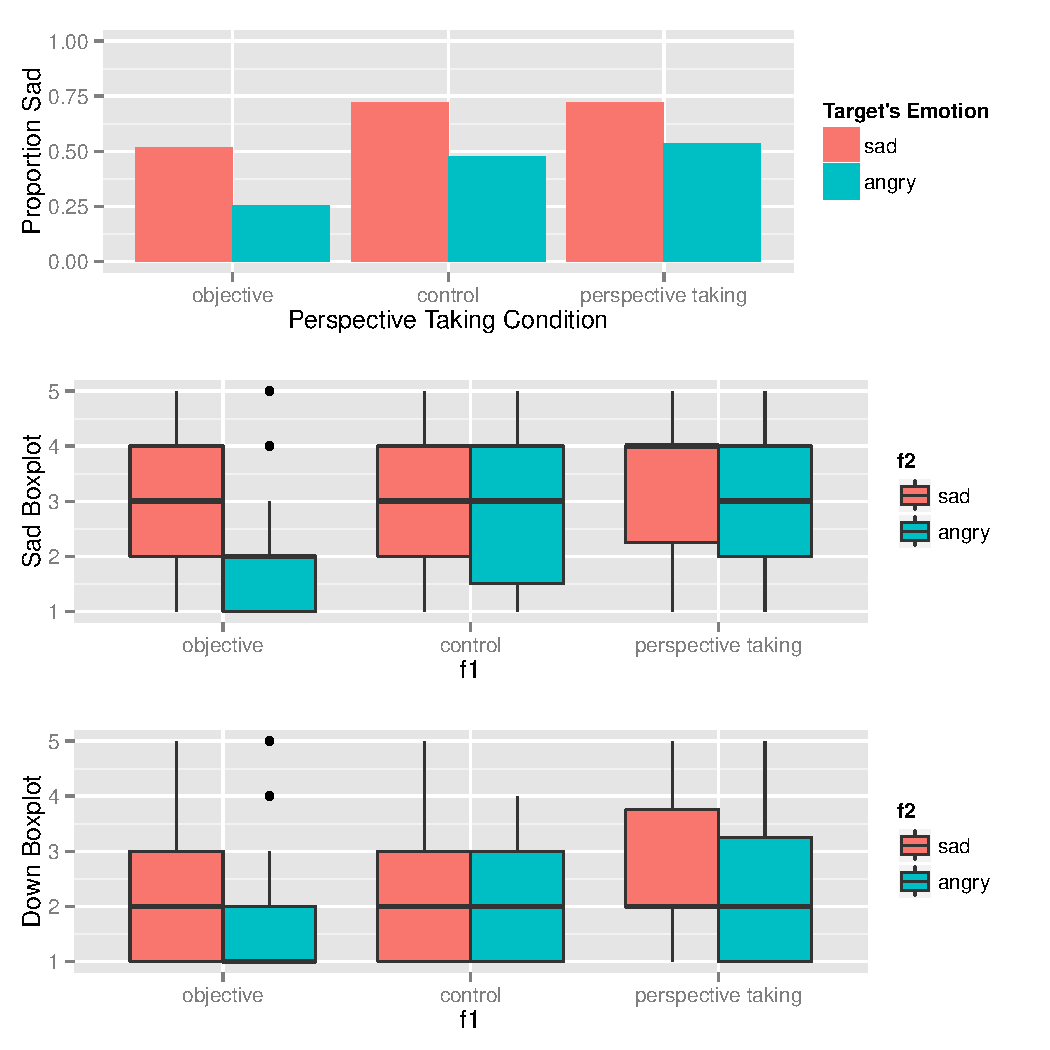
\includegraphics[width=\maxwidth]{figure/SadPlot} 

\end{knitrout}
\textit{Figure 1.} Subjects' sadness by condition.
\end{figure}

\subsection{Anger}    


Figure 2 displays subjects' anger in the open-ended and closed-ended data. 
    Subjects were more likely to report that they felt angry when they read an angry letter from Melissa (35\%) than when they read an angry letter from Melissa (14\%) in their open-ended responses, 95\% CI [0.3, 0.86]. They also reported feeling more angry, 95\% CI [0.29, 0.72], and mad, 95\% CI [0.25, 0.67], in the closed-ended data.
    For subjects who read the angry letter, subjects were no more likely to report that they felt angry when they took Melissa's perspective (45\%) than in the control condition (39\%) in the open-ended data, 95\% CI [-0.25, 0.5]; they also reported feeling equally angry, 95\% CI [-0.05, 0.62], and mad, 95\% CI [-0.09, 0.58], in the closed-ended data. Those who remained objective were equally likely to report that they felt angry (22\%) to those in the control condition in the open-ended data, 95\% CI [0, 0.83]. However, they reported feeling less angry, 95\% CI [0.17, 0.87], and mad, 95\% CI [0.24, 0.94], in the closed-ended data. Those who remained objective also reported feeling less angry than those who took Melissa's perspective in the open-ended data, 95\% CI [0.12, 0.96], and less sad, 95\% CI [0.45, 1.16], and down, 95\% CI [0.47, 1.19], than those who took Melissa's perspective in the closed-ended data.
    Once again, there was no evidence that perspective taking caused subjects to feel angry like Melissa, but there was evidence that remaining objective caused them to feel less angry.
    
\begin{figure}
\begin{knitrout}
\definecolor{shadecolor}{rgb}{0.969, 0.969, 0.969}\color{fgcolor}\begin{kframe}


{\ttfamily\noindent\color{warningcolor}{\#\# Warning: Removed 1 rows containing non-finite values (stat\_boxplot).}}\end{kframe}
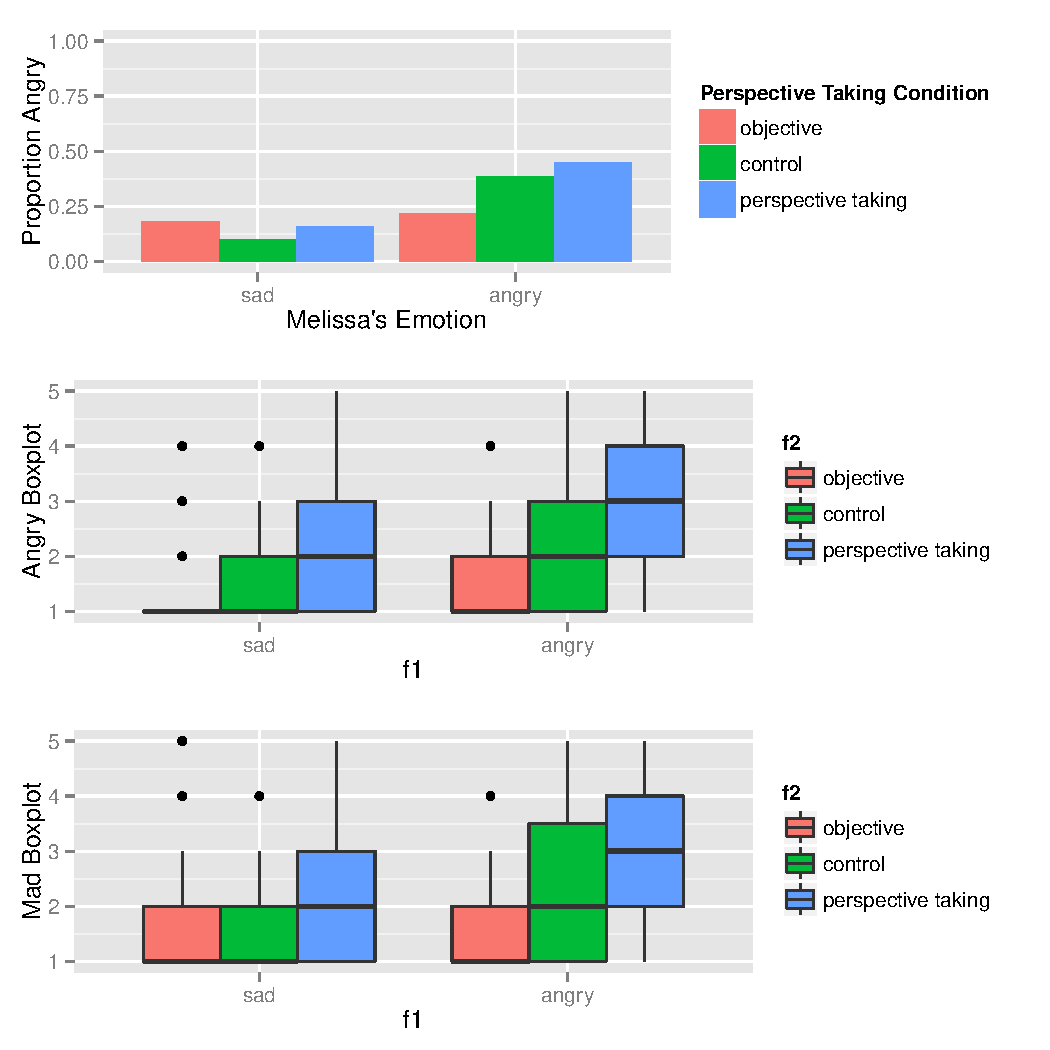
\includegraphics[width=\maxwidth]{figure/AngerPlot} 

\end{knitrout}
\textit{Figure 2.} Subjects' anger by condition.
\end{figure}

\subsection{Did Perspective Taking Make Subjects More Likely to Feel Emotions that Melissa Did Not Feel?}

Another way to understand whether perspective taking makes people feel how the target of perspective taking feels is to see if the effects are emotion-specific. In other words, if there are differences in anger across conditions, do those differences only occur when the other person is angry? We examined differences in sadness when subjects read an angry letter and differences in anger when subject read a sad letter.
    For subjects who read an angry letter, they were as likely to report feeling sad when they took Melissa's perspective (54\%) as in the control condition (47\%) in the open-ended data, 95\% CI [-0.24, 0.5], and they were equally likely to report feeling sad, 95\% CI [-0.21, 0.45], and down, 95\% CI [-0.64, -0.2]. However, they were less likely to report feeling sad when they remained objective (25\%) than in the control condition in the open-ended data, 95\% CI [0.09, 0.89], and they reported feeling less sad, 95\% CI [0.24, 0.94], and less down 95\% CI [0.13, 0.87], in the closed-ended data. Those who remained objective also reported feeling less sad than those who took Melissa's perspective in the open-ended data, 95\% CI [0.22, 1.02], and less sad, 95\% CI [0.37, 1.06], and less down, 95\% CI [0.4, 1.14], in the closed-ended data.
    For subjects who read a sad letter, they were as likely to report feeling angry when they took Melissa's perspective (16\%) as in the control condition (10\%) in the open-ended data, 95\% CI [-0.25, 0.5], and they were equally likely to report feeling angry, 95\% CI [-0.05, 0.62], and mad, 95\% CI [-0.09, 0.58]. They were also as likely to report feeling angry when they remained objective (18\%) as when they took Melissa's perspective, 95\% CI [-0.59, 0.44], or were in the control condition, 95\% CI [-0.92, 0.19] in the open-ended data. They were also equally likely to report feeling angry, 95\% CI [0.17, 0.87], and mad, 95\% CI [0.24, 0.94], as those in the control condition in the closed-ended data; however, they felt less angry, 95\% CI [0.45, 1.16], and less mad, 95\% CI [0.47, 1.19], than those in the perspective taking condition.
    In summary, there was some evidence that those who remained objective not only felt what Melissa felt less than those in the perspective taking and control conditions, but they also felt the opposite emotion less, though the results were more consistent for subjects' sadness after reading an angry letter than for subjects' anger after reading a sad letter. 

\subsection{Did Perspective Taking Make Subjects More Sympathetic?}


    Although some theories have proposed that perspective taking makes people more empathetic, meaning they feel what the perspective taking target feels, a lot of empirical research has focused on feelings of sympathy-concern for the perspective taking target that is not necessarily the same emotion as what the target feels. Even though we found no evidence that perspective taking increased empathy, might it increase subjects' sympathy?
    Figure 3 displays subjects' sympathy in the open-ended and closed-ended data. Overall, subjects were equally likely to say that they felt sympathetic when they read a sad letter (60\%) and when they read an angry letter (68) in their open-ended responses. They also reported feeling equally sympathetic in the closed-ended data, 95\% CI [-0.28, 0.12]; however, those read a sad letter felt more compassionate than those who read an angry letter, 95\% CI [-0.43, -0.04].
    For subjects who read a sad letter, subjects were equally likely to say that they felt sympathetic when they took Melissa's perspective (74\%) and when they were in the control condition (72\%) in their open-ended responses, 95\% CI [-0.37, 0.48]. Similarly, they were equally likely to feel sympathetic, 95\% CI [-0.13, 0.6], and compassionate, 95\% CI [-0.17, 0.51], in their closed-ended responses. They were also as likely to say that they felt sympathetic when they remained objective (57\%) as those who took Melissa's perspective, 95\% CI [-0.03, 0.8], or were in the control condition, 95\% CI [-0.05, 0.72]. They also reported feeling as compassionate as those in the control condition, 95\% CI [-0.11, 0.53], in the closed-ended data. However, those who remained objective felt less compassionate than subjects who took Melissa's perspective, 95\% CI [0.04, 0.72], and they felt less sympathetic than those who took Melissa's perspective, 95\% CI [0.36, 1.08], and those who were in the control condition, 95\% CI [0.15, 0.83].
    For subjects who read an angry letter, subjects were equally likely to say that they felt sympathetic when they took Melissa's perspective (61\%) and when they were in the control condition (70\%) in their open-ended responses, 95\% CI [-0.61, 0.18]. Similarly, they were equally likely to feel sympathetic, 95\% CI [-0.17, 0.53], and compassionate, 95\% CI [-0.04, 0.64], in their closed-ended responses. They were also as likely to say that they felt sympathetic when they remained objective (49\%) as those who took Melissa's perspective, 95\% CI [-0.14, 0.62], in their open-ended responses; however, those who remained objective were less likely to feel sympathetic than those in the control condition, 95\% CI [0.06, 0.84]. Those who remained objective also reported feeling less sympathetic than those who took Melissa's perspective, 95\% CI [0.39, 1.09], or were in the control condition, 95\% CI [0.29, 0.99], and they felt less compassionate than those who took Melissa's perspective, 95\% CI [0.39, 1.09], and those who were in the control condition, 95\% CI [0.1, 0.78].
    Once again, there was little evidence that perspective taking increased sympathy, but more evidence that remaining objective decreased it.

    
\begin{figure}
\begin{knitrout}
\definecolor{shadecolor}{rgb}{0.969, 0.969, 0.969}\color{fgcolor}\begin{kframe}


{\ttfamily\noindent\color{warningcolor}{\#\# Warning: Removed 2 rows containing non-finite values (stat\_boxplot).}}\end{kframe}
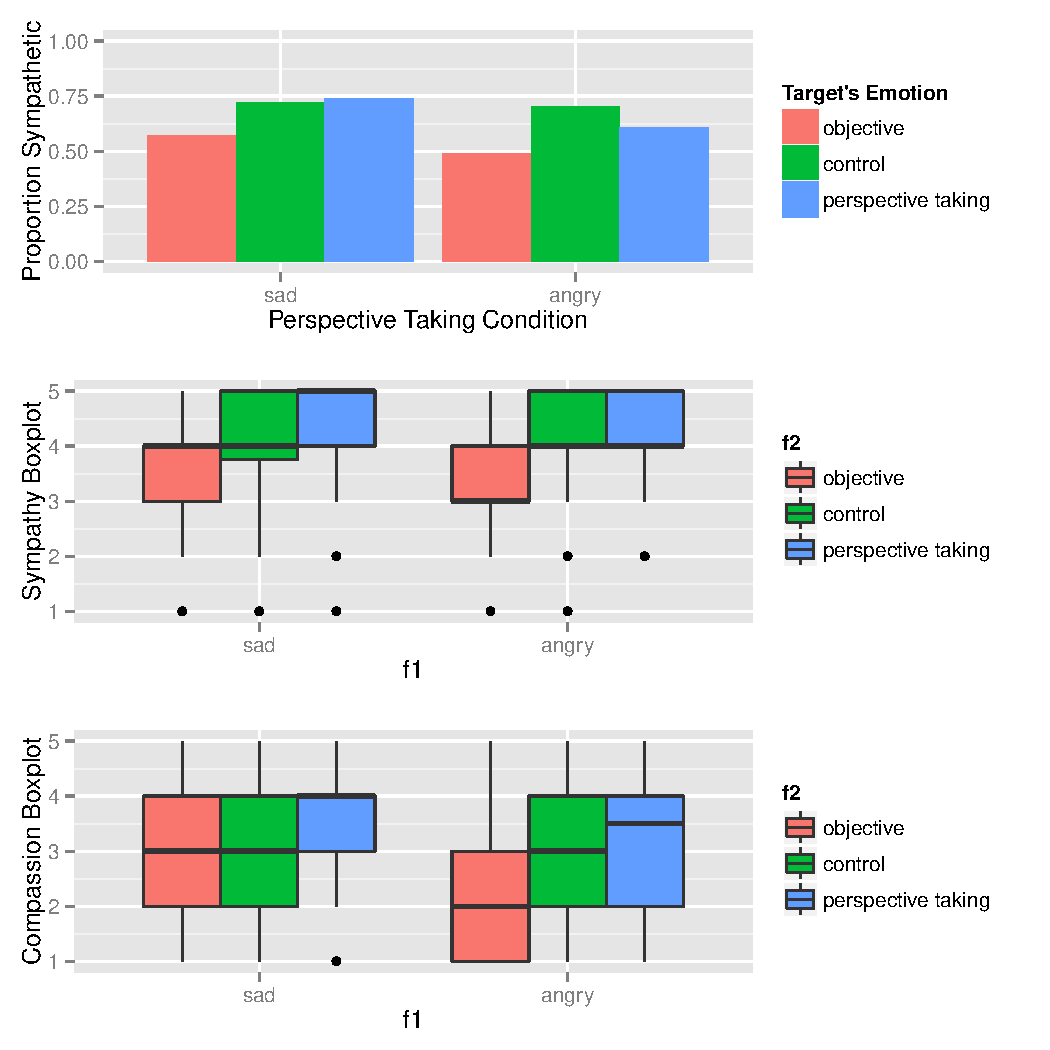
\includegraphics[width=\maxwidth]{figure/SympPlot} 

\end{knitrout}
\textit{Figure 3.} Subjects' sympathy by condition.
\end{figure}


\bibliography{ptreferences}
\bibliographystyle{apacite}

\end{document}
